\documentclass[border=10pt]{standalone}
\usepackage[T1]{fontenc}
\usepackage{tikz}
\usepackage{amsmath}

\definecolor{garnet}{HTML}{73000A}
\definecolor{atlantic}{HTML}{466A9F}
\definecolor{congaree}{HTML}{1F414D}
\definecolor{warmgrey}{HTML}{676156}
\definecolor{horseshoe}{HTML}{65780B}
\definecolor{bk70}{HTML}{5C5C5C}
\definecolor{bk30}{HTML}{C7C7C7}
\definecolor{bk10}{HTML}{ECECEC}

\begin{document}
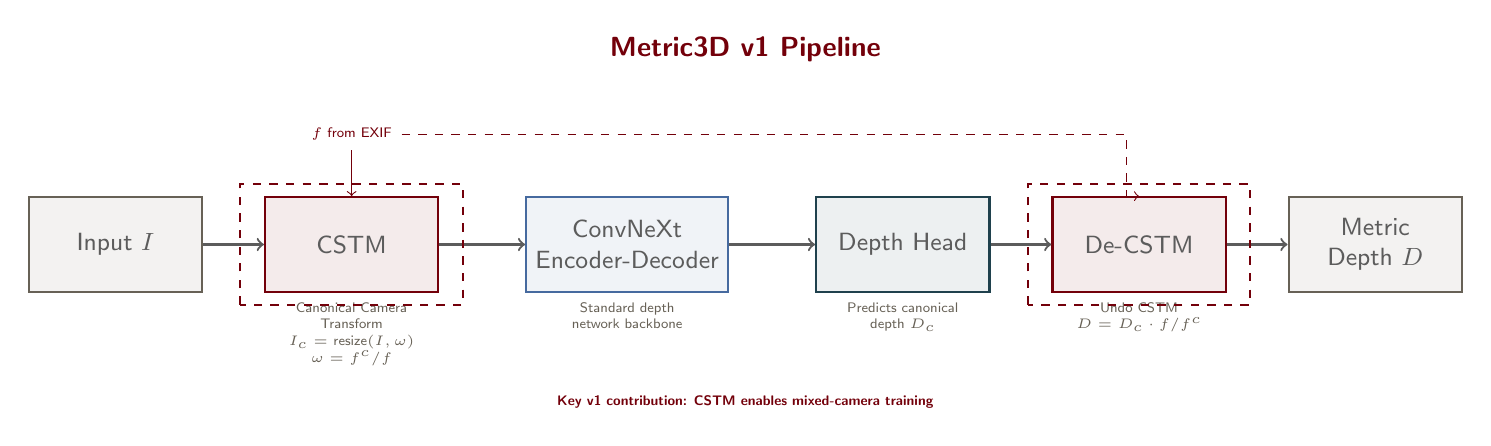
\begin{tikzpicture}[
    block/.style={
        draw=#1, thick, fill=#1!8,
        minimum height=1.2cm, minimum width=2.2cm,
        font=\sffamily\small, text=bk70, align=center,
    },
    arr/.style={->, thick, color=bk70},
    label/.style={font=\sffamily\tiny, text=warmgrey, align=center},
]

% ── v1 Pipeline blocks ──
% Input
\node[block=warmgrey] (input) at (0, 0) {Input $I$};

% CSTM
\node[block=garnet] (cstm) at (3, 0) {CSTM};

% Encoder-Decoder
\node[block=atlantic] (backbone) at (6.5, 0) {ConvNeXt\\Encoder-Decoder};

% Depth head
\node[block=congaree] (dhead) at (10, 0) {Depth Head};

% De-CSTM
\node[block=garnet] (decstm) at (13, 0) {De-CSTM};

% Output
\node[block=warmgrey] (output) at (16, 0) {Metric\\Depth $D$};

% ── Arrows ──
\draw[arr] (input) -- (cstm);
\draw[arr] (cstm) -- (backbone);
\draw[arr] (backbone) -- (dhead);
\draw[arr] (dhead) -- (decstm);
\draw[arr] (decstm) -- (output);

% ── Annotations below ──
\node[label, anchor=north] at (cstm.south) {Canonical Camera\\Transform\\$I_c = \text{resize}(I, \omega)$\\$\omega = f^c / f$};

\node[label, anchor=north] at (backbone.south) {Standard depth\\network backbone};

\node[label, anchor=north] at (dhead.south) {Predicts canonical\\depth $D_c$};

\node[label, anchor=north] at (decstm.south) {Undo CSTM\\$D = D_c \cdot f / f^c$};

% ── Focal length input ──
\node[font=\sffamily\tiny, text=garnet, anchor=south] (flabel) at (3, 1.2) {$f$ from EXIF};
\draw[->, thin, garnet] (flabel) -- (cstm.north);
\draw[->, thin, garnet, dashed] (flabel.east) -- ++(9.2,0) |- (decstm.north);

% ── Title ──
\node[font=\sffamily\bfseries, text=garnet, anchor=south] at (8, 2.2) {Metric3D v1 Pipeline};

% ── Key contribution highlight ──
\draw[garnet, thick, dashed] ([xshift=-0.3cm, yshift=-0.15cm]cstm.south west)
    rectangle ([xshift=0.3cm, yshift=0.15cm]cstm.north east);
\draw[garnet, thick, dashed] ([xshift=-0.3cm, yshift=-0.15cm]decstm.south west)
    rectangle ([xshift=0.3cm, yshift=0.15cm]decstm.north east);

\node[font=\sffamily\tiny\bfseries, text=garnet, anchor=north] at (8, -1.8)
    {Key v1 contribution: CSTM enables mixed-camera training};

\end{tikzpicture}
\end{document}
